\clearpage
\section*{二、实验操作与原始数据}

\subsection*{1. 实验操作与原始记录}

用于标称电容可能不准或已经被击穿，正式实验前需要用 LCR 电表测量电容，再组成七个补偿档位。电源设为220 V，按50、45、55 Hz的顺序测量，每种频率记录八组数据。

同一频率下，我依次测量未加电容及各补偿档位的电流、电压、功率和功率因数。以下为原始记录及转录表。

\begin{figure}[H]\centering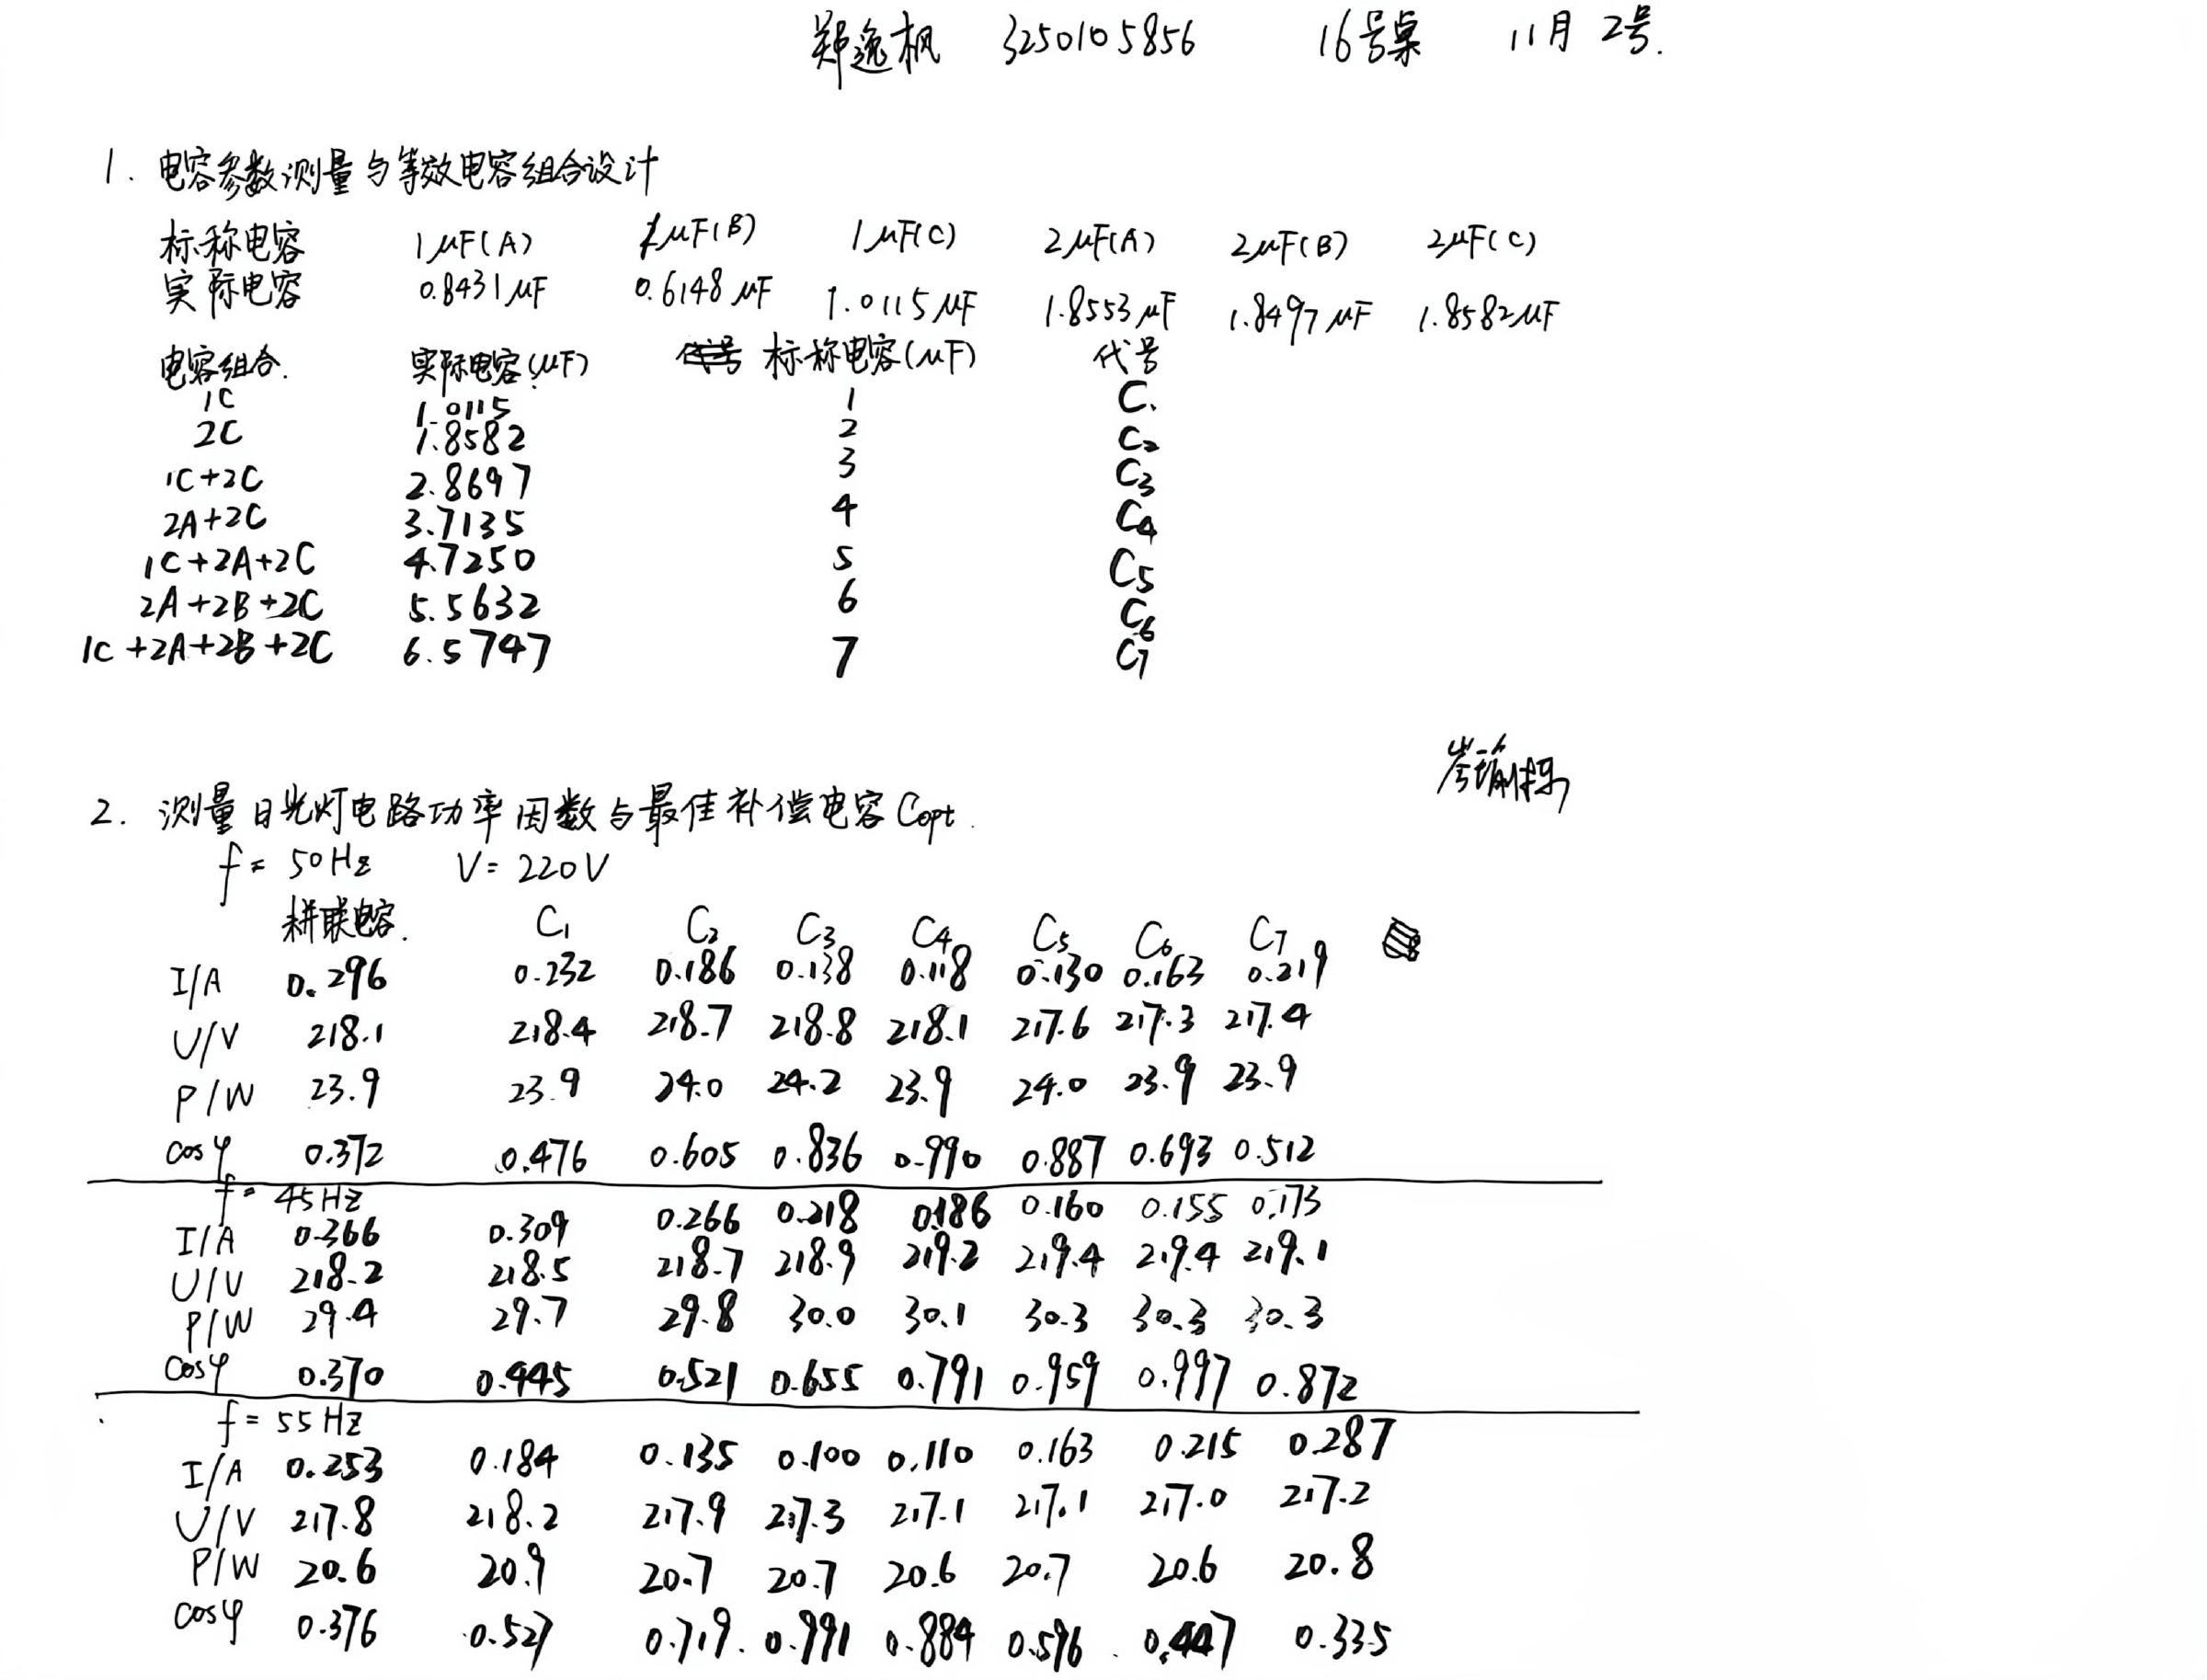
\includegraphics[width=16cm]{../assets/raw-data.png}\caption{本次原始记录（已按阅读方向旋转）}\end{figure}

\subsection*{2. 电容参数与组合}

1A表示标称1 μF的A号电容，其余类推。各电容的实测值如下。

\begin{center}\small
\begin{tabular}{ccccccc}
\toprule
电容编号 & 1A & 1B & 1C & 2A & 2B & 2C \\
\midrule
实测值/μF & 0.8431 & 0.6148 & 1.0115 & 1.8553 & 1.8497 & 1.8582 \\
\bottomrule\end{tabular}\end{center}

\clearpage

各档电容均采用并联组合，编号及电容值如下。

\begin{center}\small
\begin{tabular}{cccc}
\toprule
档位 & 并联组合 & 标称值/μF & 实际值/μF \\
\midrule
$C_1$ & 1C & 1 & 1.0115 \\
$C_2$ & 2C & 2 & 1.8582 \\
$C_3$ & 1C+2C & 3 & 2.8697 \\
$C_4$ & 2A+2C & 4 & 3.7135 \\
$C_5$ & 1C+2A+2C & 5 & 4.7250 \\
$C_6$ & 2A+2B+2C & 6 & 5.5632 \\
$C_7$ & 1C+2A+2B+2C & 7 & 6.5747 \\
\bottomrule\end{tabular}\end{center}

\subsection*{3. 三种频率下的测量数据}

表内均为现场测量值，电压为实测值。

\textbf{50 Hz：}

\begin{center}\small
\begin{tabular}{ccccccccc}
\toprule
量 & 未加电容 & $C_1$ & $C_2$ & $C_3$ & $C_4$ & $C_5$ & $C_6$ & $C_7$ \\
\midrule
$I$/A & 0.296 & 0.232 & 0.186 & 0.138 & 0.118 & 0.130 & 0.163 & 0.219 \\
$U$/V & 218.1 & 218.4 & 218.7 & 218.8 & 218.1 & 217.6 & 217.3 & 217.4 \\
$P$/W & 23.9 & 23.9 & 24.0 & 24.2 & 23.9 & 24.0 & 23.9 & 23.9 \\
$\cos\varphi$ & 0.372 & 0.476 & 0.605 & 0.836 & 0.990 & 0.887 & 0.693 & 0.512 \\
\bottomrule\end{tabular}\end{center}

\textbf{45 Hz：}

\begin{center}\small
\begin{tabular}{ccccccccc}
\toprule
量 & 未加电容 & $C_1$ & $C_2$ & $C_3$ & $C_4$ & $C_5$ & $C_6$ & $C_7$ \\
\midrule
$I$/A & 0.266 & 0.309 & 0.266 & 0.218 & 0.186 & 0.160 & 0.155 & 0.173 \\
$U$/V & 218.2 & 218.5 & 218.7 & 218.9 & 219.2 & 219.4 & 219.4 & 219.1 \\
$P$/W & 29.4 & 29.7 & 29.8 & 30.0 & 30.1 & 30.3 & 30.3 & 30.3 \\
$\cos\varphi$ & 0.370 & 0.445 & 0.521 & 0.655 & 0.791 & 0.959 & 0.997 & 0.872 \\
\bottomrule\end{tabular}\end{center}

\textbf{55 Hz：}

\begin{center}\small
\begin{tabular}{ccccccccc}
\toprule
量 & 未加电容 & $C_1$ & $C_2$ & $C_3$ & $C_4$ & $C_5$ & $C_6$ & $C_7$ \\
\midrule
$I$/A & 0.253 & 0.184 & 0.135 & 0.100 & 0.110 & 0.163 & 0.215 & 0.287 \\
$U$/V & 217.8 & 218.2 & 217.9 & 217.3 & 217.1 & 217.1 & 217.0 & 217.2 \\
$P$/W & 20.6 & 20.9 & 20.7 & 20.7 & 20.6 & 20.7 & 20.6 & 20.8 \\
$\cos\varphi$ & 0.376 & 0.527 & 0.719 & 0.991 & 0.884 & 0.586 & 0.447 & 0.335 \\
\bottomrule\end{tabular}\end{center}



